\documentclass{article} % For LaTeX2e
\usepackage{../../tex-style/nips_2014,times}
\usepackage{hyperref}
\usepackage{url}
\usepackage{graphicx}
\usepackage{CJKutf8}
\hypersetup{unicode}
\AtBeginShipoutFirst{\input{zhwinfonts.tex}}
\usepackage{algorithm}  
\usepackage{algorithmic}
\usepackage{amsmath}
\title{Neural Networks and Physical Systems with Emergent Collective Computational Abilities}

\author{
 \url{https://www.dosrc.com/}
}


\nipsfinalcopy % Uncomment for camera-ready version

\begin{document}
\begin{CJK*}{UTF8}{gkai}

\maketitle

\section{Hopfield networks}
\subsection{网络结构}
\begin{center}
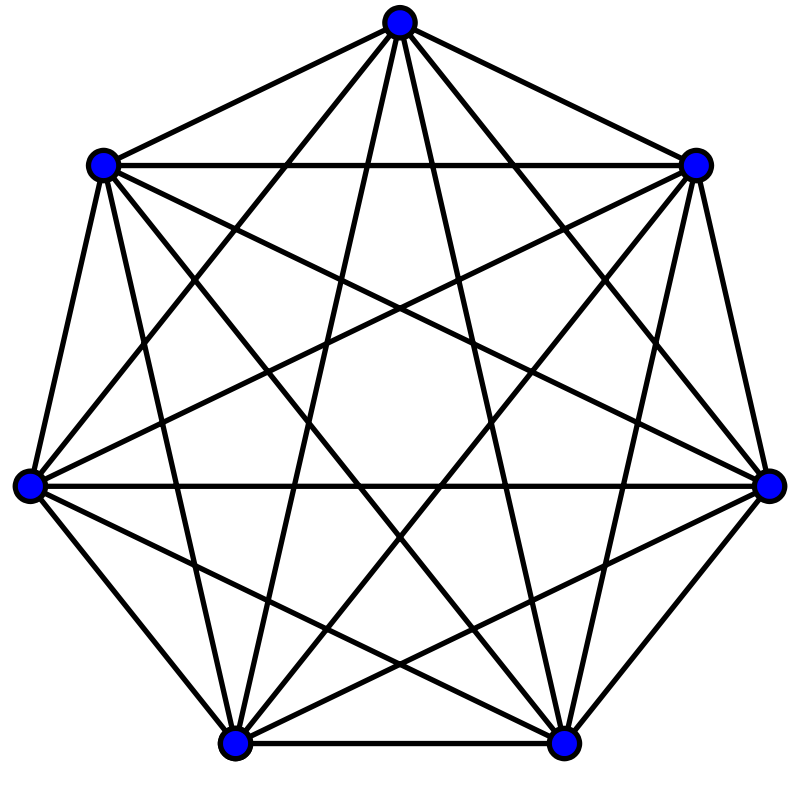
\includegraphics[width=2in]{complete-graph.png}
\end{center}
网络结构由完全图构成,即各个神经元之间互相连接并有权重代表他们之间的连接强度,每个神经元输出1或0(或者1/-1)这两个值,神经元依然有阈值,超过阈值输出1,否则为0,神经元的输出是其它神经元的输出加权和,即$ V _{j}^{\prime} = f \left( \sum _{j \neq i} T _{ij} V _{j} \right) $,其中$T _{ij}$为神经元$i$到$j$之间的权重,$V _{j}$为神经元$j$的输出。更新神经元的输出时不能同时更新所有神经元的输出否者可能会导致震荡,当权值固定并且对称时($T _{ij}=T _{ji}$)网络最终会到达一个稳定的状态,此时我们称网络的能量达到了局部最小值,权值不对称时,网络可能到达震荡甚至混乱的状态。当$T _{ij}=T _{ji}$时,网络的能量定义如下:
$$ E = -\dfrac{1}{2} \sum _{i}\sum _{j} T _{ij}V _{i} V _{j}.$$
所以给定所有的神经元一个初始的值,该神经网络最终会达到能量局部最低的状态,整个网络就像一个动力系统,倾向于保持能量处于一个较小的状态。就像物理学中水往低处走的现象。能量的局部极小值可能有很多个,给定神经元以不同的初始值能量可能会收敛到不同的局部最小值。给极小值附近的点施加一个轻微的扰动,它还是会回到极小值点,由于该神经网络的这个特点,我们可以把它用在联想记忆上。\textbf{联想记忆系统}存储着一系列记忆向量的集合。只要给联想记忆网络一个相关的记忆向量,他就能正确恢复出原来存储的记忆向量,例如联想记忆系统存储着一句话,我们可能只需要几个词语它就能联想起整句话。

\subsection{学习规则}
要让上述网络存储不同的记忆向量,就要让这些需要记忆的向量都变成能量方程的局部最小值点。所以我们就得寻找一种方法可以让任意点都成为局部极小值点。
此外学习规则还需要满足以下两条性质:

1. local 即某个权重的更新要只依赖与它相邻的两个神经元

2. Incremental 能增量学习,即记忆某个新模式(向量)不必依赖原来的向量,权重的更新只依赖于它的旧值和新的要记忆的模式

\subsubsection{Hebbian learning rule for Hopfield networks}
当神经元输出0/1时:
$$ T _{ij} = \sum _{s}\left(2V _{i}^{s}-1\right) \left(2V _{j}^{s}-1\right)$$
当神经元输出1/-1时:
$$ T _{ij} = \sum _{s}V _{i}^{s} V _{j}^{s}$$

这个学习规则的意思是,同时激发的两个神经元倾向于形成强的连接关系。
\subsubsection{The Storkey learning rule}
略
\subsection{动力学角度的解释}
Energy Gap:
$$ \Delta E _{i} = E\left(s_{i}=0\right)-E\left(s_{i}=1\right)=\sum _{j \neq i} T _{ij} V _{j}$$
当$ \Delta E _{i} < 0$时$\sum _{j \neq i} T _{ij} V _{j} < 0$说明当($s_{i}=0$)时整个网络的能量比($s_{i}=1$)小,所以令$s_{i}=0$

当$ \Delta E _{i} > 0$时$\sum _{j \neq i} T _{ij} V _{j} > 0$说明当($s_{i}=0$)时整个网络的能量比($s_{i}=1$)大,所以令$s_{i}=1$

这正好符合更新规则
\subsection{储存效率}
对一个N个神经元的上述网络,它大概能存储$M=0.15N$个记忆向量,再多就会产生混乱,每个记忆向量为N位(例如1000个神经元的上述网络能存储150个记忆向量,每个记忆向量为1000位),所有总共存储了$0.15N ^{2}$个bit

但是构建一个这样的网络所需要的存储量为:$N^{2}$个权重,每个权重的值为$[-M, M]$其中$M$为存储的记忆向量的个数,所以需要$N^{2}\times log(2M+1)$位来存储这些权重
\begin{center}
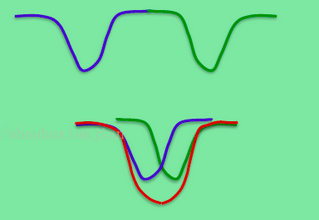
\includegraphics[width=2in]{misrepresentation.png}
\end{center}
\end{CJK*}
\end{document}